Para iniciar la ejecución, una vez hemos ingresado a la plataforma y
estamos en la nube, debemos ver una imagen similar a la siguiente:

\begin{figure}[ht!]
	\centering
	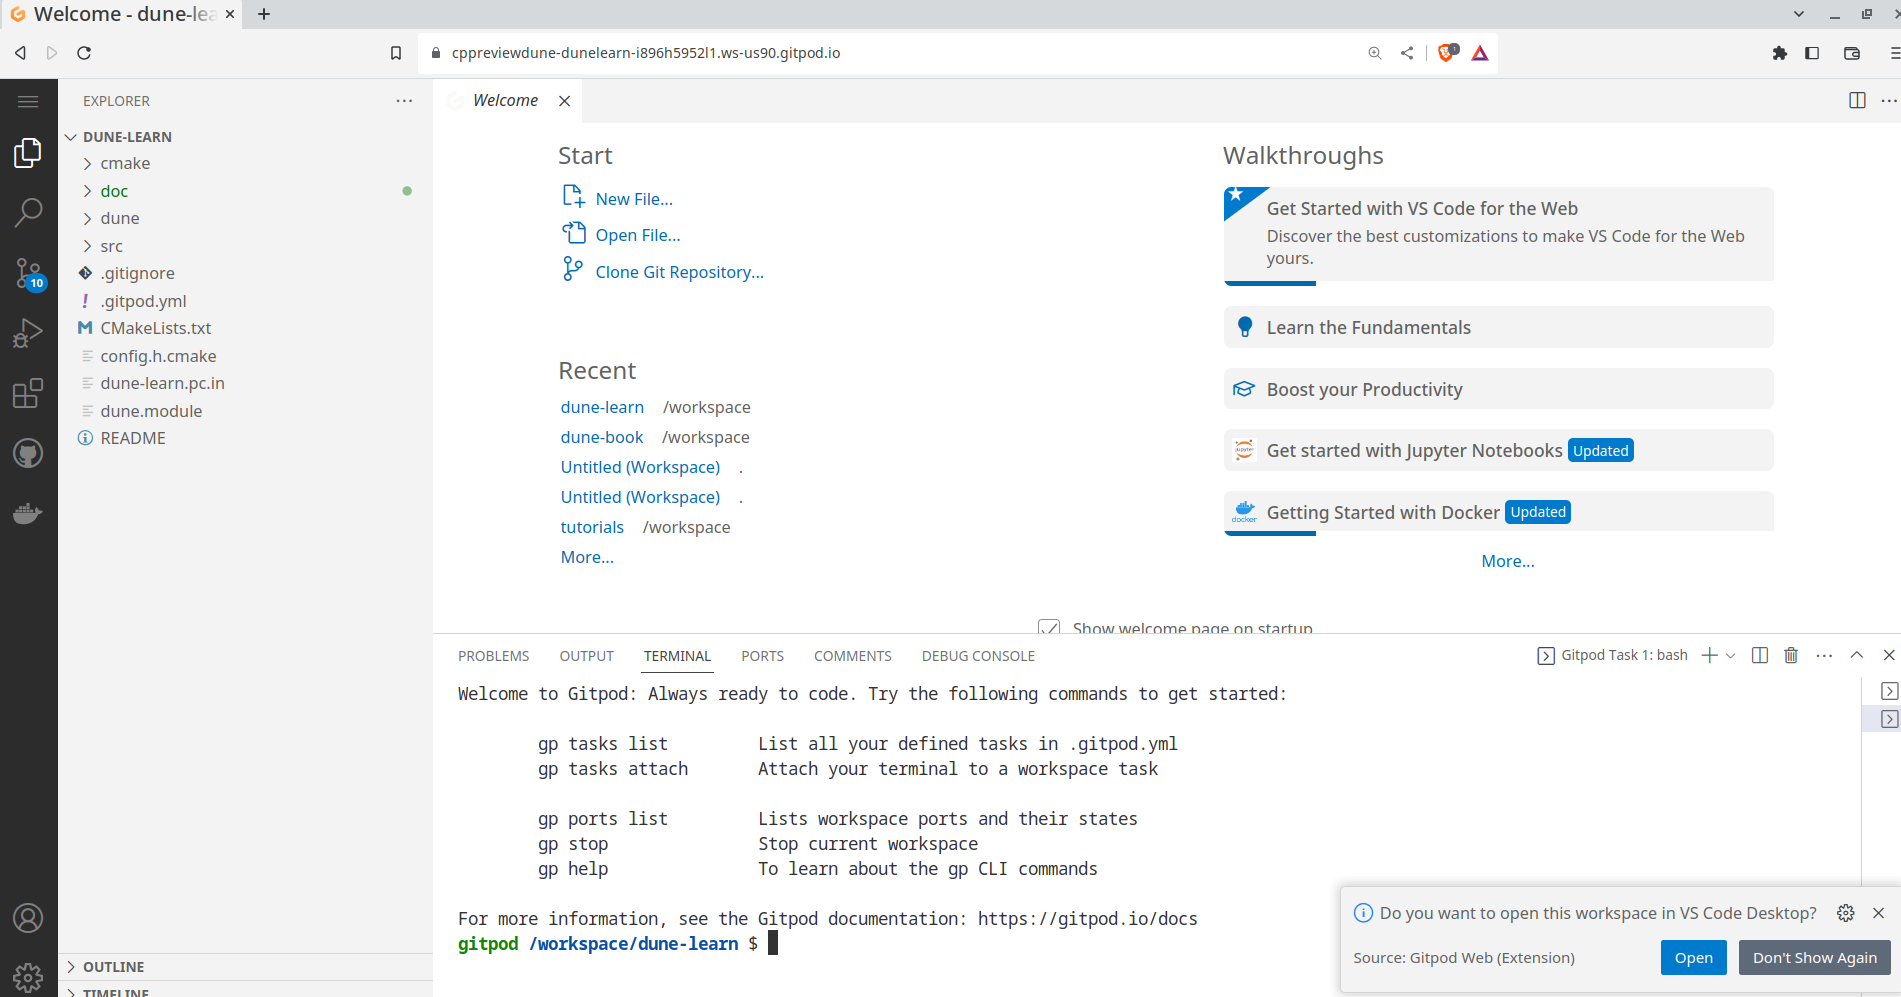
\includegraphics[scale=0.3,keepaspectratio]{PantallaIngreso.png}
	\label{fig:ingreso}
\end{figure}

Como se puede apreciar, es muy similar al editor de código basado en
navegador, \href{https://microsoft.github.io/monaco-editor}{Monaco}.
Para hacer mi primer proyecto, en la terminal debo escribir:

\textcolor{green}{gitpod}\textcolor{blue}{/workspace}\$ duneproject
\begin{verbatim}

== Dune project/module generator ==

duneproject will assist you in the creation of a new Dune application.
During this process a new directory with the name of your project will be
created. This directory will hold all configuration and Makefiles and a
simple example application.

1) Name of your new Project? (e.g.: dune-grid): 
\end{verbatim}

En ésta parte, debo completar la información de mi proyecto, el
nombre vamos a poner por ejemplo \verb|dune-prueba|, luego

\begin{verbatim}
  2) Which modules should this module depend on?
   The following modules have been found:
   dune-common dune-geometry dune-uggrid dune-grid dune-localfunctions dune-istl 
   dune-typetree dune-functions dune-alugrid dune-pdelab dune-fem dune-learn 
   Enter space-separated list:
\end{verbatim}

En éste caso, vamos a usar \verb|dune-pdelab|, luego pregunta:

\begin{verbatim}
  3) Project/Module version? 
\end{verbatim}

Por ejemplo puede ser $01$, luego nos pide el email:

\begin{verbatim}
  4) Maintainer's email address? maintainer@unal.edu.co 
\end{verbatim}

Finalmente, nos pregunta si los datos están correctos:

\begin{verbatim}
  creating Project "dune-prueba", version 01 
which depends on "dune-pdelab"
with maintainer "maintainer@unal.edu.co"
Is this information correct? [y/N] y
\end{verbatim}

Si los datos son correctos, asignamos ``y'', de lo contrario ``N'', y
finalmente enter para iniciar la configuración.
Una vez iniciada la configuración, se crea una carpeta con el nombre
\verb|dune-prueba|, que fue el nombre del proyecto que asignamos.
Una vez que el proyecto se ha construido, podemos utilizar el comando
\begin{verbatim}
gitpod/workspace $ ls
\end{verbatim}

Dentro del listado debe aparecer la carpeta
\textcolor{blue}{dune-prueba}, que si explora dentro de ella,
encontrará varios archivos y carpetas.
Se puede dirigir a la siguiente dirección:
\begin{verbatim}
cd /workspace/dune-prueba/src $ 
\end{verbatim}
Cuando liste, encontrará dos archivos

\begin{verbatim}
CMakeLists.txt  dune-prueba.cc
\end{verbatim}

En el primer archivo, usted encuentra lo siguiente:

\begin{verbatim}
add_executable("dune-prueba" dune-prueba.cc)
target_link_dune_default_libraries("dune-prueba")
\end{verbatim}

Significa que se ha creado un código fuente, que se llama
``dune-prueba.cc'', tiene el mismo nombre del proyecto que creamos, y
en el que está escrito nuestro primer programa, el ``Hola mundo de DUNE''.
A continuación se puede apreciar el contenido completo del primer programa:

\begin{listing}
	\inputminted{cpp}{../../src/dune-learn.cc}
\end{listing}

\immediate\write18{./run.sh}